\chapter{An All-Sky Multi-flare Analysis}\label{chapter:multiflareskymap}

\section{Motivation}
While the previous section outlined the application of the multi-flare algorithm to a pair of source catalogs, an additional obvious application of the method is to simply apply the algorithm across the entire neutrino sky. While catalog searches have the advantage of a greatly reduced trial factor, they also rely on having a mostly-correct guess of the underlying source population. By contrast, an all-sky search could potentially reveal sources without requiring any prior knowledge of what the specific sources could be, and could additionally even identify astrophysical neutrino sources with no multi-messenger counterpart. Given the results of a temporally untriggered neutrino flare associated with TXS 0506+056~\cite{TXS_Archival}, it is only natural to ask whether other such flares exist in IceCube's astrophysical neutrino data. An all-sky multi-flare analysis would be an appropriate approach of detecting a population of TXS-like flares, should they exist. 

Similar to the FAVA analysis produced by the Fermi collaboration~\cite{fava_paper}, an IceCube multi-flare skymap provides a description of the temporal variability of every point in the sky. Even in the absence of a statistically significant population of neutrino flares, these neutrino "flare curves" may be of use for multi-messenger analyses in the future, similar to what was done for TXS 0506+056~\cite{TXS_Archival}\cite{TXS_Multimessenger}.

\section{Analysis Construction}
Conceptually, the construction of an all-sky multi-flare analysis is fairly straightforward: a grid of pixels with  is defined over the entire sky using the \texttt{HEALPY} software package~\cite{healpy2019}. Using a \textt{HEALPY} grid with a \texttt{Nside=256} results in a grid of $786,432$ pixels, each with a radius of $0.12^{\circ}$. Pixels with declinations $\delta>85^{\circ}$ or $\delta<-85^{\circ}$ are excluded, as the data-driven method of estimating background using data scrambled in right ascension does not perform well in this region due to the small statistics of declination bands near the poles. The multi-flare algorithm is then applied to the central location of each pixel, resulting in a map of multi-flare test statistics, each associated with an individual pixel. 

The significance of each pixel can then be calculated by comparing the observed multi-flare test statistic to a distribution of similar test statistics obtained by applying the above procedure to maps of IceCube events that have had their right ascension locations randomized, providing a description of the null hypothesis. Pixels are divided into 40 declination bands, and for each declination band a chi-squared distribution is fit to the distribution of test statistics in that declination range. A pre-trial local significance for each pixel is calculated by comparing a particular pixel test statistic to the chi-squared distribution that was fit in the corresponding declination band. Once this has been done for every pixel, a map of multi-flare p-values has been obtained, describing the local multi-flare significance of every pixel in the sky.

Once a p-value map has been generated, several basic tests can be conducted. The most obvious test is to simply check if the most significant pixel is more significant than is expected from the background case (a "hotspot" test). A distribution of most significant multi-flare p-values is created by applying the procedure above to a set of background maps. The most significant pixel in the observed multi-flare map can then be compared to this distribution to obtain a final hotspot significance that has been trial-corrected for the all sky trial factor. As the event selection is different in the northern and southern skies, this process is conducted separately for declinations $\delta>-5^{\circ}$ and $\delta<-5^{\circ}$

Populations of multi-flare sources may also be tested for using a binomial test. A set of "spatially independent" local hotspots may be obtained by defining a list of all pixels that are at least $1^{\circ}$ away from a more significant pixel. The binomial test statistic p-value of the population test is then defined as (eq.~\ref{eq:bitest}):

\begin{equation}
    p(k) = \sum_{i=k}^{N_{eff}} \binom{N_{eff}}{i}p_k^i(1-p_k)^{N_{eff}-i}
    \label{eq:bitest}
\end{equation}

Here, $p(k)$ is correlated with the significance of observing $k$ hot spots with a p-value of $p_k$ or less, and $N_{eff}$ is the effective number of trials associated with the list of hot spots, chosen to produce proper containment of the final binomial p-values (e.g. a final binomial p-value of $p=0.1$ or less should only occur in 10\% of background trials). In this case, $N_{eff}=N_{pixels}$ produces proper containment. Hot spots are ordered by decreasing significance, and $k$ is varied to identify the most significant combination. The $p(k)$ associated with the best fit $k$ is then compared to a distribution of $p(k)$'s obtained in a similar manner from data scrambled in right ascension, resulting in a final post-trial binomial p-value. Like with the study of the most significant pixel, this process is conducted separately in the northern and southern skies. 

Since the multi-flare algorithm fits for every flare candidate at a particular pixel, it is trivial to extract the single-flare skymap results from this process as well. The procedure is almost identical to that which was outlined above, except instead of using the multi-flare test statistic at each pixel, the test statistic of the flare with the highest test statistic at each pixel is used. The hotspot and population tests then proceed as normal.

This particular analysis uses the PSTracksv003p02 data set.

\section{Results}
\subsection{Hotspots and Populations Analysis}
The multi-flare pre-trial p-value map can be seen in figure~\ref{fig:mfskymap}, with the locations of the brightest multi-flare pixels marked. The most significant locations identified by the multi-flare algorithm have pre-trial p-values of $p=9.2\times10^{-6}$, located at (RA, Dec)=$(145.02^{\circ}, 36.42^{\circ})$ and $p=3.5\times10^{-7}$, located at (RA, Dec)=$(126.21^{\circ}, -24.81^{\circ})$. These pre-trial p-values can be corrected to account for the all-sky trial factor using the process described above, resulting in post-trial p-values of $p=0.69$ for the northern sky hot spot and $p=0.06$ for the southern sky hot spot.

\begin{figure}[h]
\centering
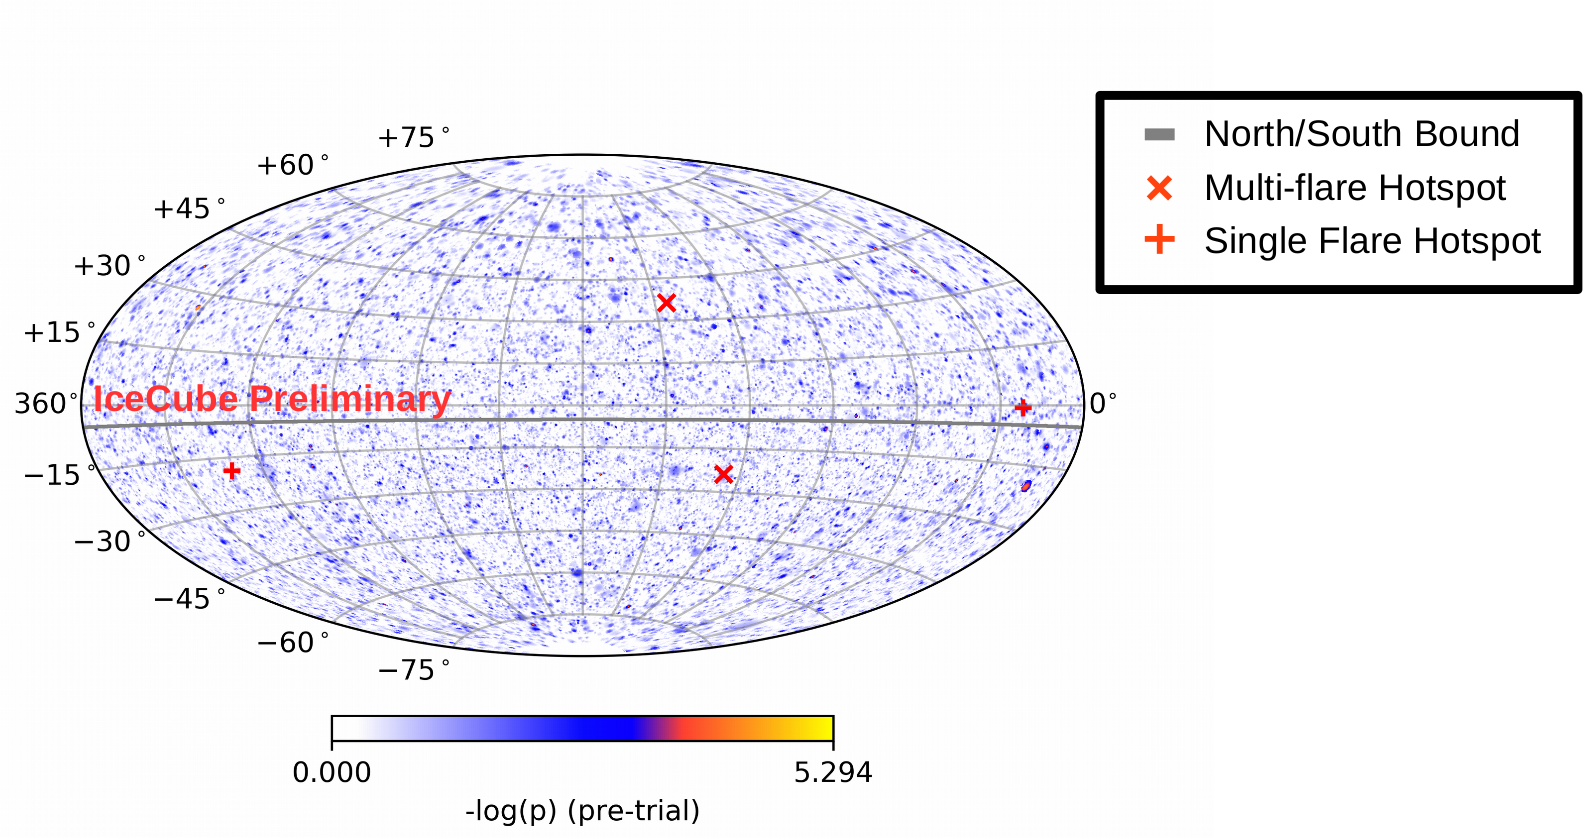
\includegraphics[width=0.8\textwidth]{figs/skymap_withlabels.png}
\caption{The p-value map produced by applying the multi-flare algorithm to the entire neutrino sky between $-85^{\circ}<\delta<85^{\circ}$. The locations of the most significant multi-flare pixels in each hemisphere are shown as red "$\times$'s", while the locations of the most significant individual flares in each hemisphere are shown as red "$+$'s". The gray line denotes the boundary between what is considered the "northern" and "southern" sky by the IceCube data sample that was used. }
\label{fig:mfskymap}
\end{figure}

The flare curves for the multi-flare hotspots can be seen in figure~\ref{fig:mfhotspots}. Note that the multi-flare test statistic is a measure of the activity of a source integrated over the entire livetime of the data sample. While no individual flares that were fit at either the northern or southern hotspot are particularly significant on their own, the combination of many moderately significant flares is what makes these pixels the brightest multi-flare pixels in their respective hemispheres. 

\begin{figure}[h]
\centering
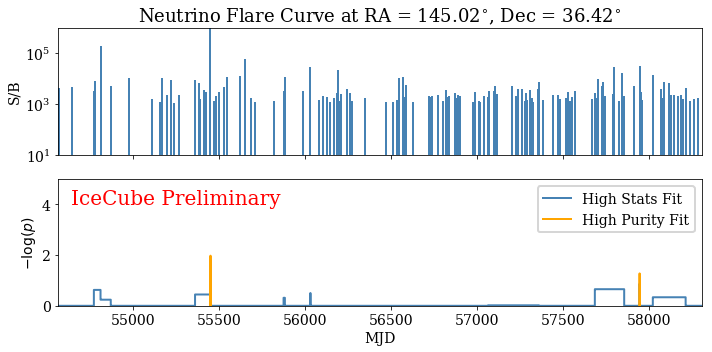
\includegraphics[width=0.4\textwidth]{figs/fcurve_mf_north.png}
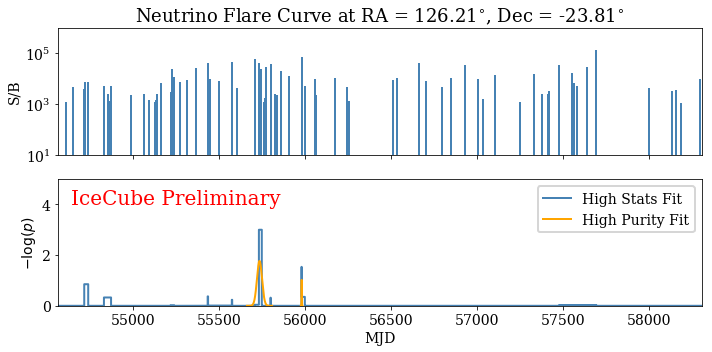
\includegraphics[width=0.4\textwidth]{figs/fcurve_mf_south.png}
\caption{The flare curves returned by the multi-flare algorithm for the most significant pixel in the northern sky (left), and southern sky (right). For comparison, a complementary high-purity fit that uses a gaussian hypothesis and more stringent cuts on flare decorrelation is shown in orange. In both the northern and southern sky, the multi-flare significance is fueled not by individual flares with high local significance, but rather by a large number of moderately significanct flares. }
\label{fig:mfhotspots}
\end{figure}

Since the application of the high-statistics multi-flare analysis involves fitting every possible flare in the data, it is trivial to additionally calculate the significance of the largest individual flare candidate that was fit in both the northern and southern sky. We find that the most significant flare candidate in the northern sky is located at (RA, Dec)=$(21.97^{\circ}, -0.60^{\circ})$ (recall that the "northern sky" refers to declinations between $-5^{\circ}$ and $85^{\circ}$), and has a pre-trial significance of $p=5.08\times10^{-6}$ ($p=0.82$ post-trial). The most significant flare candidate in the southern sky is located at (RA, Dec)=($311.66^{\circ}, -18.84^{\circ}$), and has a pre-trial significance of $p=6.8\times10^{-6}$ ($p=0.53$ post-trial). 

\begin{figure}[h]
\centering
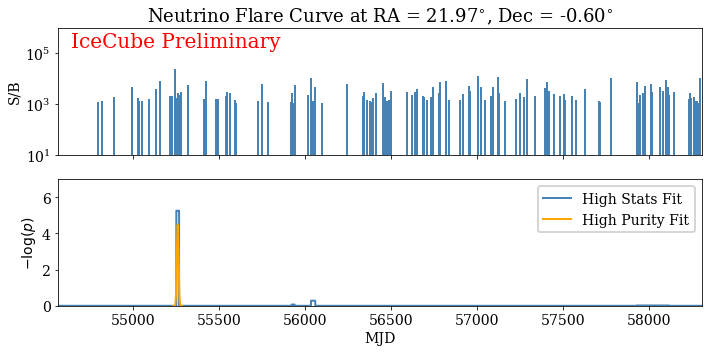
\includegraphics[width=0.4\textwidth]{figs/fcurve_sf_north.png}
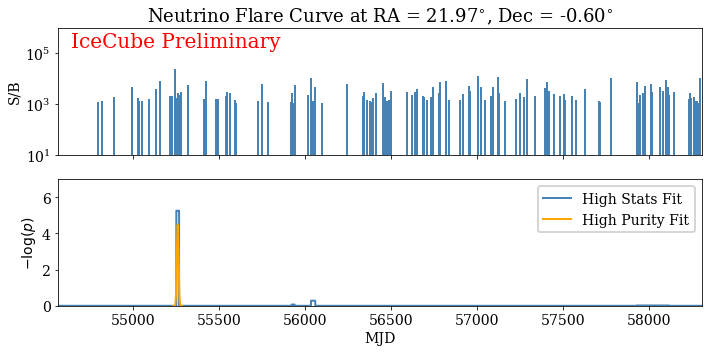
\includegraphics[width=0.4\textwidth]{figs/fcurve_sf_north.png}
\caption{The flare curves returned by the multi-flare algorithm for the most significant flares identified in the northern sky (left), and southern sky (right). For comparison, a complementary high-purity fit that uses a gaussian hypothesis and more stringent cuts on flare decorrelation is shown in orange. Since neither of these locations appear to display significant activity beyond the large individual flares, these do not constitute particularly significant locations from a multi-flare perspective.}
\label{fig:mfhotspots}
\end{figure}

In addition to examining the most significant pixels that were seen, it is also informative to conduct a population analysis on the set of spatially independent ($>1^{\circ}$ separation) hotspots using the binomial test framework described above. In both the northern and southern sky, the binomial test was conducted for the set of spatially independent hotspots, defined by both the local multi-flare and single-flare significance. In all cases, the best-fit combination of hotspots was $k=1$, tagging only the most significant pixel, and none of the associated binomial p-values were significant (results may be viewed in table~\ref{tab:popresults}).

\begin{table}[h]
\centering
\begin{tabular}{ccccc}
    %\multicolumn{5}{c}{Results}\\
    \hline
    \hline
    Analysis & Search & Hemisphere & Pre-trial p-value & Post-trial p-value\\[3pt] \hline
    \multirow{4}{*}{Multi-flare} & \multirow{2}{*}{Hottest spot} & North & $9.2\times10^{-6}$ & 0.69\\ & & South & $3.5\times10^{-7}$ & 0.06 \\ \cline{2-5}  & \multirow{2}{*}{Population test} & North & 0.98 & 0.98\\ & & South & 0.12 & 0.12\\ [3pt] \hline
    \multirow{4}{*}{Single Flare} & \multirow{2}{*}{Hottest spot} & North & $5.08\times10^{-6}$& $0.82$\\ & & South & $6.70\times10^{-6}$& $0.53$\ \\ \cline{2-5}  & \multirow{2}{*}{Population test} & North & $0.88$ & $0.88$\\ & & South & $0.91$ & $0.91$ \\
    \hline
    \hline
\end{tabular}
\caption{Summary of the tests that were performed on the unblinded multi-flare skymap. Both hotspot and population analyses were conducted using both the local multi-flare significance (summing contributions from all flare candidates at a particular location) and the local single-flare significance (taking only the largest flare fit at each location). There were no significant transient neutrino sources identified by any of the tests conducted. }
\label{tab:popresults}
\end{table}

\begin{figure}[h]
\centering
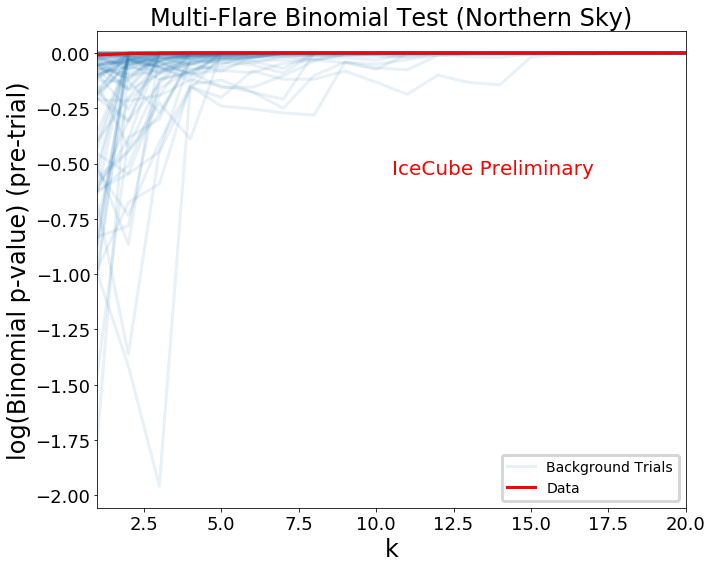
\includegraphics[width=0.4\textwidth]{figs/bicurve_north.png}
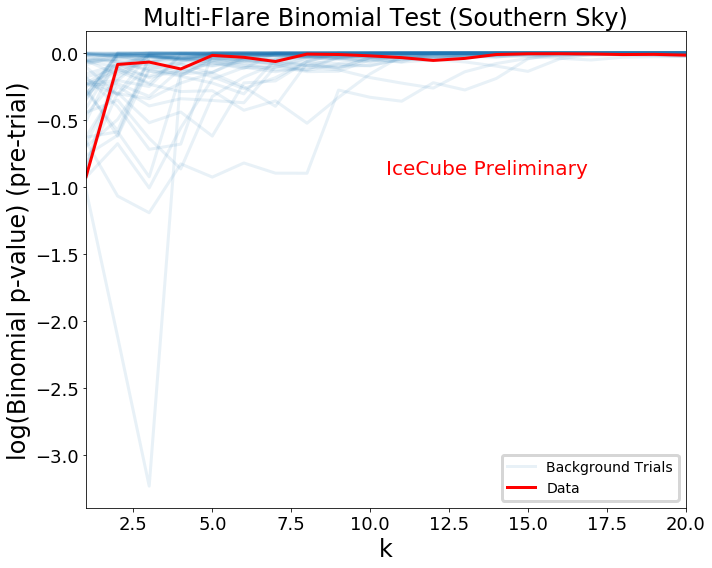
\includegraphics[width=0.4\textwidth]{figs/bicurve_south.png}
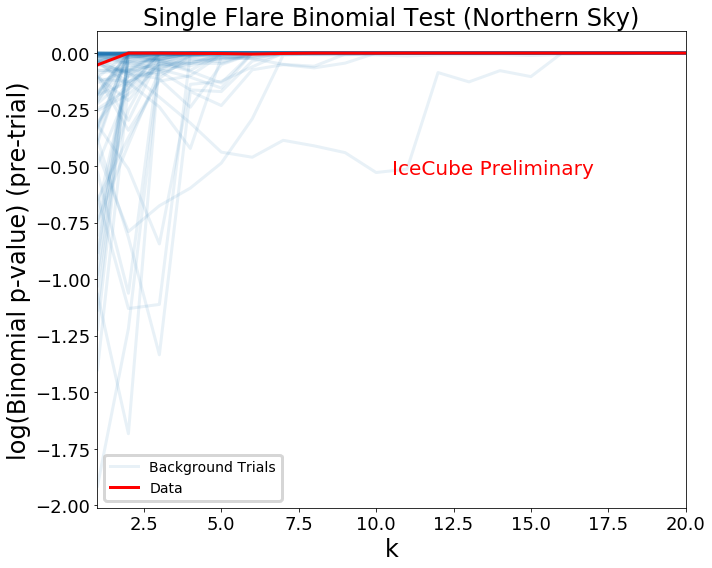
\includegraphics[width=0.4\textwidth]{figs/bicurve_sf_north.png}
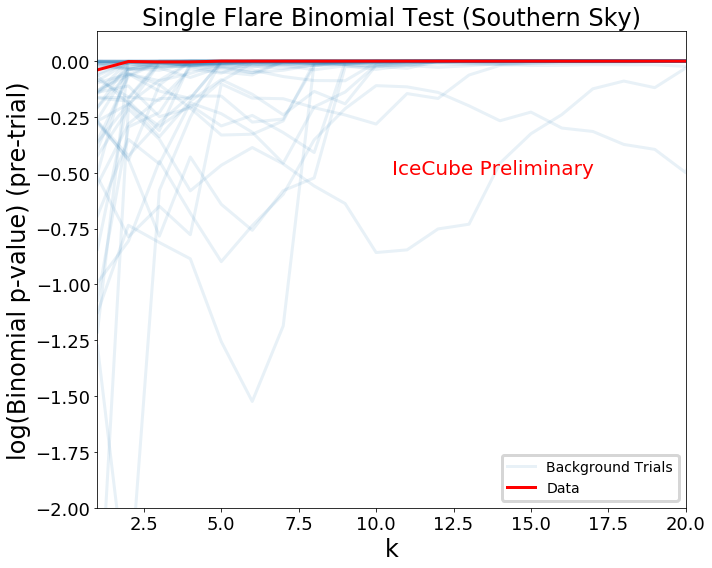
\includegraphics[width=0.4\textwidth]{figs/bicurve_sf_south.png}
\caption{The local significance of the binomial test for various values of $k$, the fitted number of hotspots, for both single and multi-flare binomial tests conducted in both the northern and southern hemispheres. Unblinded data is shown in red, while results obtained from background maps are shown in blue. In all cases using unblinded data, the observed binomial test curve has a global minimum at $k=1$, with an associated p-value that is consistent with the background expectation.}
\label{fig:bicurves}
\end{figure}

The results of the population analysis are unsurprising, given the distribution of per-pixel local p-values observed from the data. In the presence of a significant population of flaring neutrino sources, some deformation of the local p-value distribution should be visible, however as can be seen in figure~\ref{fig:pdists}, the observed distribution is entirely consistent with what is expected from background maps. 

\begin{figure}[h]
\centering
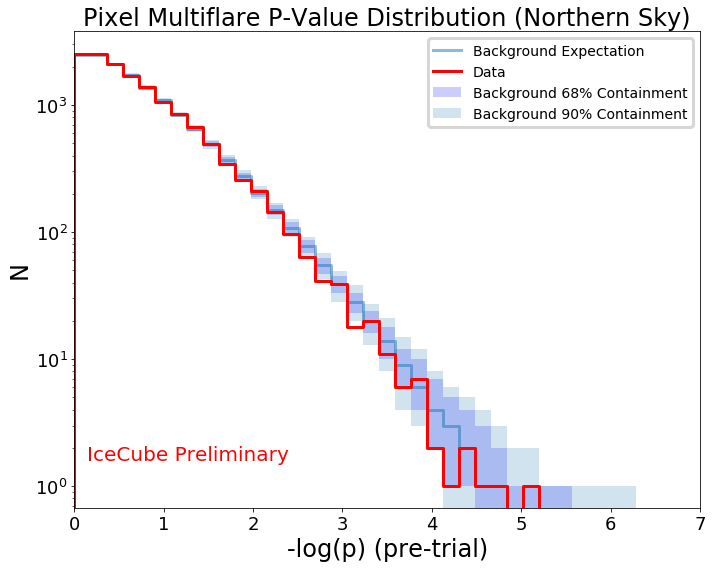
\includegraphics[width=0.4\textwidth]{figs/pixel_pdist_north.png}
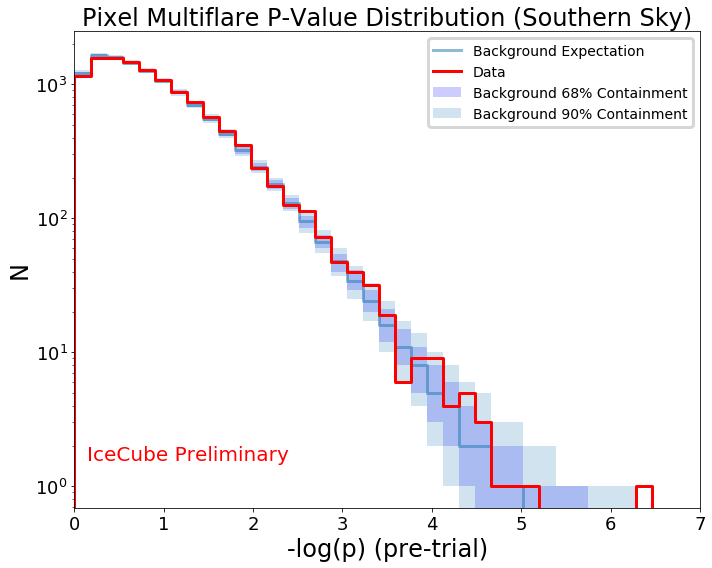
\includegraphics[width=0.4\textwidth]{figs/pixel_pdist_south.png}
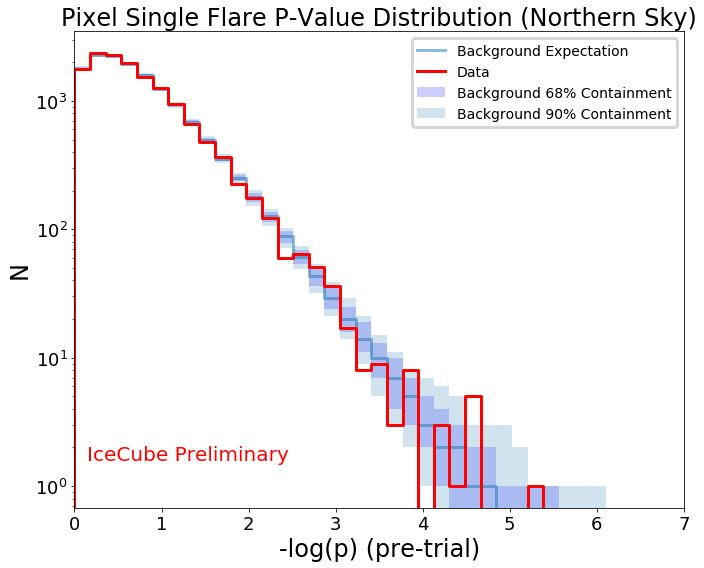
\includegraphics[width=0.4\textwidth]{figs/pixel_sf_pdist_north.png}
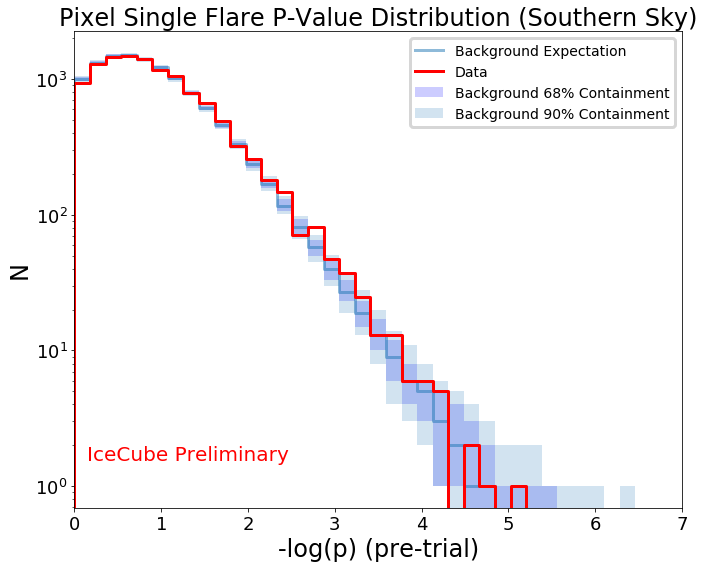
\includegraphics[width=0.4\textwidth]{figs/pixel_sf_pdist_south.png}
\caption{The local p-value distributions for the local multi-flare pixel significance (top) and the local single-flare pixel significance (bottom), for both data (red) and background maps (blue bands). In all cases, the observed distribution is consistent with the background expectation.}
\label{fig:pdists}
\end{figure}

Similar to the p-value distributions, the distributions of fitted flare parameters are also consistent with the background expectation, as can be seen in figure~\ref{fig:fitparamdists}. There does not appear to be a significant sub-population of transient sources with a particular flare duration, spectral index, flare rate, or flare flux. 

\begin{figure}[h]
\centering
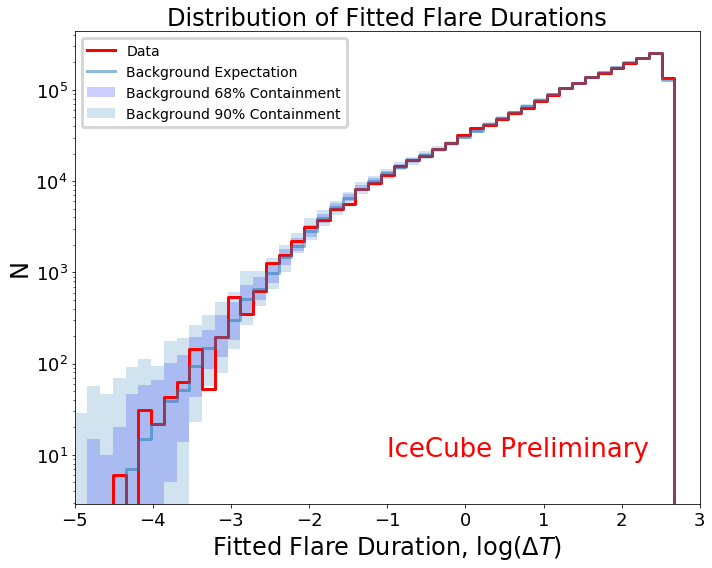
\includegraphics[width=0.4\textwidth]{figs/fitted_flare_durations.png}
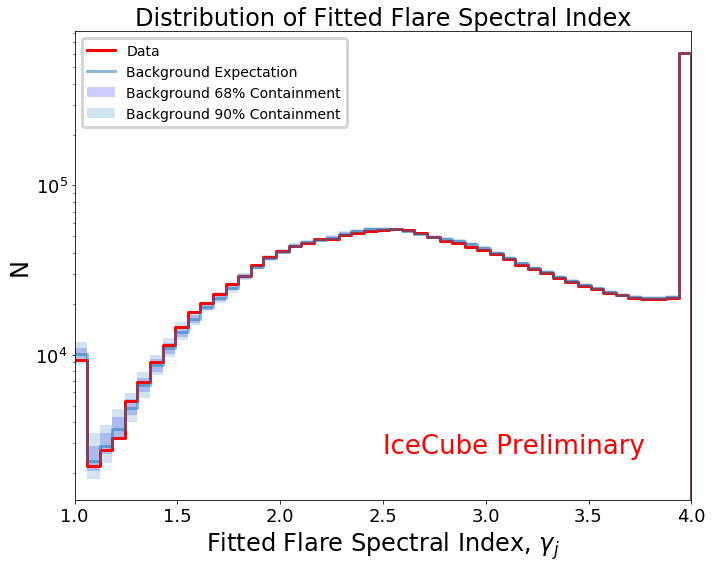
\includegraphics[width=0.4\textwidth]{figs/fitted_flare_gamma.png}
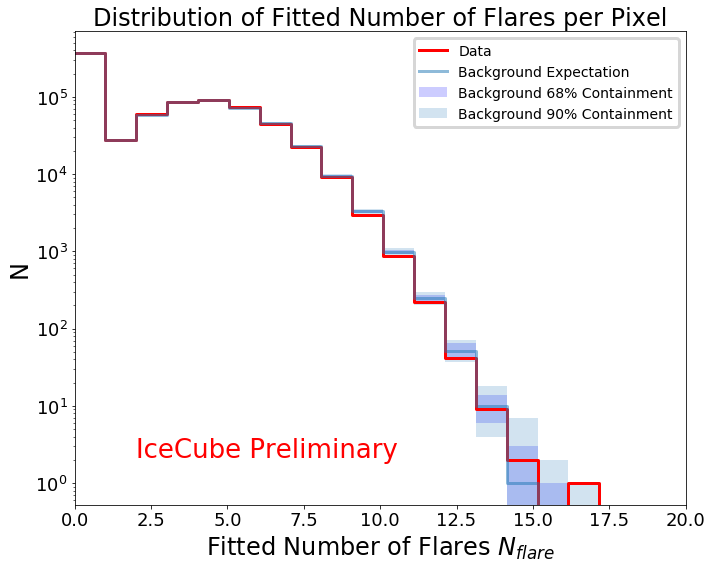
\includegraphics[width=0.4\textwidth]{figs/fitted_flare_Nflare.png}
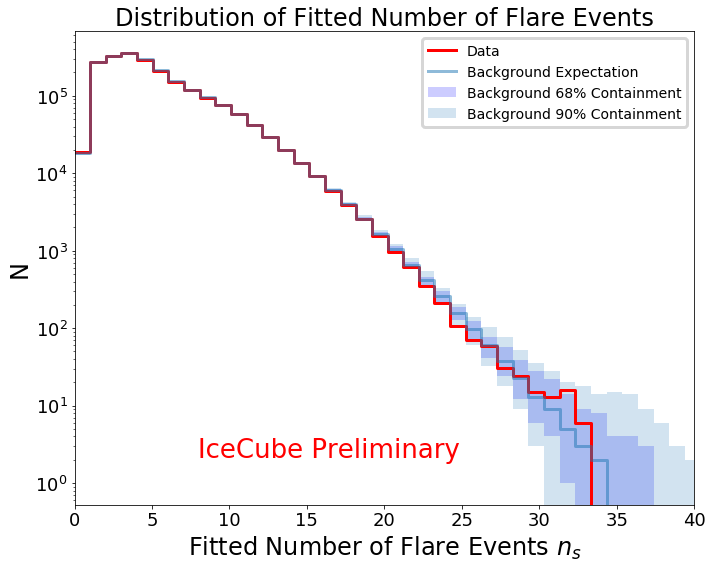
\includegraphics[width=0.4\textwidth]{figs/fitted_flare_ns.png}
\caption{Distributions of fitted flare parameters: flare duration (top, left), spectral index (top, right), number of flares fit at a particular candidate location}
\label{fig:fitparamdists}
\end{figure}

The observed diffuse astrophysical neutrino flux~\cite{stettner2019measurement} places restrictions on how bright and numerous neutrino flares may be. The non-detection of a population of transient astrophysical neutrino sources can be used to further constrain this space. These limits can be seen in figure~\ref{fig:mfskylim}, which shows 90\% upper limits on source flare rate and burst energy in neutrinos, as well as limits that can be placed on the per-source flare rate. Note that these limits are a statistical statement about the data itself: If the "true" parameters describing a population of transient neutrino sources lies above these lines, the data would have had a larger population of significant flares than what was observed. 

\begin{figure}[h]
\centering
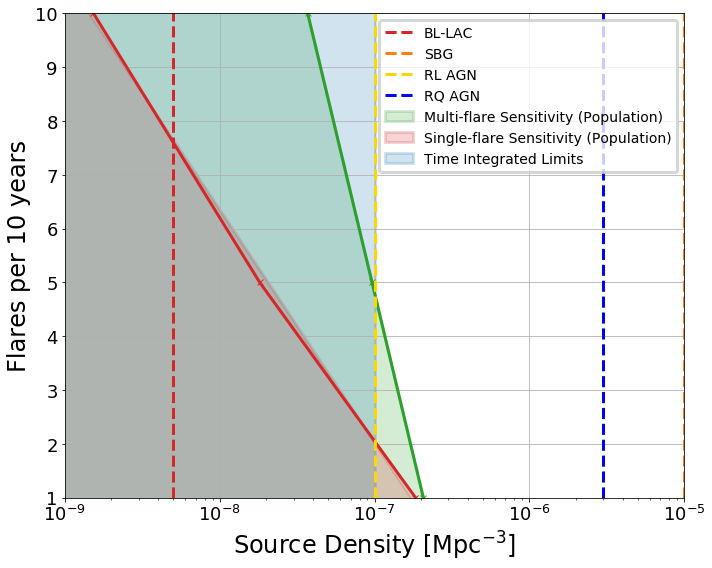
\includegraphics[width=0.4\textwidth]{figs/flarelims.png}
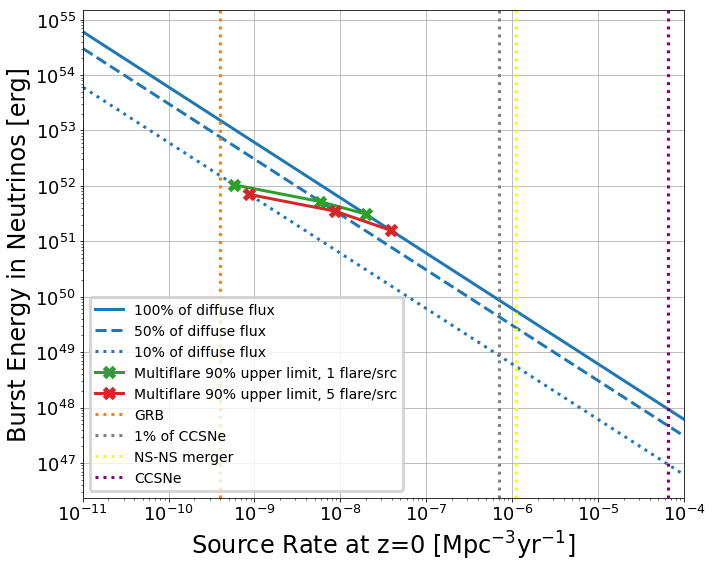
\includegraphics[width=0.4\textwidth]{figs/sourceratelims.png}
\caption{Left: 90\% upper limits on neutrino source density and per-source flare rate obtained from the all-sky multi-flare analysis. In this plot, transient sources are assumed to compose 100\% of the astrophysical neutrino flux, with the FIRESONG simulation package~\cite{firesong_ref} being used to distribute the flux among sources according to the Hopkins and Beacom (2006) source evolution model~\cite{Hopkins_2006}. Flares are simulated to have a duration of 20 days, and a spectral index of $\gamma=2.28$. All flares on the same source are assumed to have the same intrinsic intensity, equal to the time integrated source flux divided by the number of flares. Right: The 90\% upper limits on the source rate (source density $\times$ flare rate) as a function of neutrino burst energy. Blue lines correspond to combinations of source rate and neutrino burst energy that reproduce specific fractions of the diffuse astrophysical neutrino flux. In both plots, the parameters associated with several candidate source populations are shown for comparison..}
\label{fig:mfskylim}
\end{figure}


\subsection{Locations of External Interest}
Though this analysis was designed to be spatially untriggered (scanning over the entire sky, rather than the locations of a select few sources), the neutrino "flare curves" produced are a potentially powerful tool for exploring the historical behavior of source candidates identified though other methods. The skymap produced here is similar to the TXS 0506+056 followup analysis~\cite{TXS_Archival}, except that this analysis has now been performed at almost every location in the sky. This allows for easy followup of external triggers, as identifying potential transient neutrino emission associated with a source candidate is as easy as examining the flare curve at that location in the sky. 

To demonstrate the use of the all-sky flare curve map produced here, we examine the flare curves of several time-integrated source candidates identified by~\cite{10yr_tint} in order to explore the potential of temporally clustered neutrino emission from these locations. 

\subsubsection{NGC 1068}

The most significant location identified by the all-sky time-integrated analysis is spatially coincident with the Seyfert II galaxy NGC 1068. This source was also tested as part of a catalog of 110 candidate neutrino emitters, and was the brightest object in the catalog, with an associated post-trial significance of $2.9 \sigma$~\cite{10yr_tint}. These significances all arise from time-integrated tests that do not take into account the arrival time of the contributing neutrino events. It is then potentially interesting to explore the temporal structure of this excess with the flare curves that were produced as part of the multi-flare skymap. 

The flare curve generated at the location of NGC 1068 can be seen in figure~\ref{fig:ngc1068}. Though this location is significant under the time-integrated analysis, the multi-flare p-value is only $p=0.016$ (pre-trial), with no individual flare candidate having a local significance greater than $p=0.072$. Note however, that these results are not in tension with the time-integrated significance, as the time-integrated analysis tests only for an excess of events over the entire livetime of the sample. By contrast, a source with high multi-flare significance requires that events not only be clustered spatially, but temporally as well. As such, sources with high time-integrated significance do not necessarily have a correspondingly high multi-flare significance, particularly if there is not significance temporal clustering of events that contribute to the time-integrated result. 

Nonetheless, we have here provided a description of the historical behavior of the neutrino emission associated with NGC 1068. Despite the time-integrated excess observed in previous analyses, there does not appear to be significant temporal clustering of events at this location.

\subsubsection{Other Time-Integrated Candidates: PKS 1424+240  and GB6 J1542+6129}
In addition to identifying NGC 1068 as a potential source candidate, the population analysis component of the time integrated analysis~\cite{10yr_tint} also identified an excess of $3.3 \sigma$ associated with the combination of the sources NGC 1068, TXS 0506+056, PKS 1424+240, and GB6 J1542+6129. Figure~\ref{fig:othertints} shows the flare curves that were obtained at the locations of PKS 1424+240 and GB6 J1542+6129. 

Similar to NGC 1068, PKS 1424+240 does not display significant temporal clustering of neutrino events, and has a local multi-flare p-value of $p=0.085$. By contrast, GB6 J1542+612 seems to have a somewhat significant flare candidate beginning at MJD=57564.878 and ending at MJD=57944.512. The pre-trial significance of this flare candidate alone is $p=0.00173$ ($2.9 \sigma$). Combining all the flares candidates at the location of GB6 J1542+612 using the multi-flare test statistics results in a local multi-flare significance of $p=0.0098$ ($2.3 \sigma$). While this is not particularly significant (especially when the all-sky trial factor is considered), it does inform us that the period between MJD=57564.878 and MJD=57944.512 was likely a large contributor to the time-integrated significance for this particular source. If there are further multi-messenger signals from this location in the future, the neutrino flare candidates at this location may become of interest. 

\begin{figure}[h]
\centering
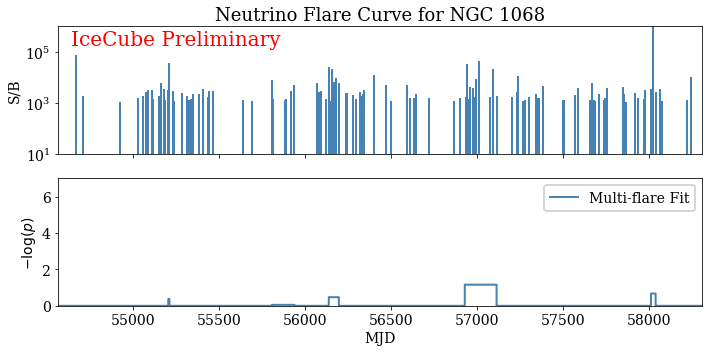
\includegraphics[width=0.8\textwidth]{figs/fcurve_NGC1068.png}
\caption{The flare curve at the location of NGC 1068, a source candidate that was identified as potentially interesting in the time-integrated analysis~\cite{10yr_tint}. While this is the brightest spot in the time-integrated analysis, the multi-flare analysis does not reveal any significant temporal clustering of events at this location, resulting in a local multi-flare significance of $p=0.016$}
\label{fig:ngc1068}
\end{figure}

\begin{figure}[h]
\centering
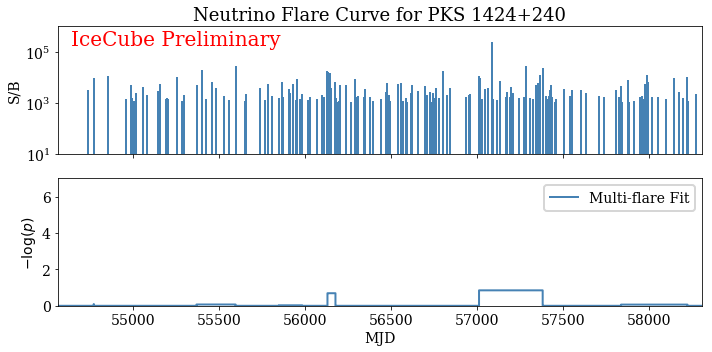
\includegraphics[width=0.4\textwidth]{figs/fcurve_PKS1424+240.png}
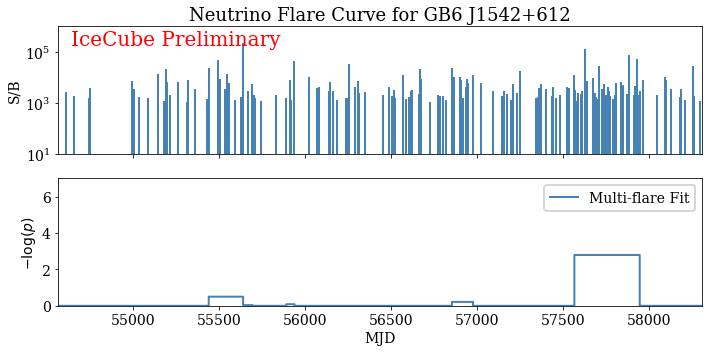
\includegraphics[width=0.4\textwidth]{figs/fcurve_GB6.png}
\caption{The flare curves at the locations of PKS 1424+240 and GB6 J1542+612. While PKS 1424+240 does not display any significant temporal clustering (having a local multi-flare p-value of $p=0.085$), GB6 J1542+612 has a potentially interesting flare candidate beginning at MJD=57564.878 and ending at MJD=57944.512. This flare candidate has a local flare significance of $p=0.00173$ ($2.9 \sigma$), contributing to the overall pre-trial multi-flare significance for GB6 J1542+612 of $p=0.0098$ ($2.3 \sigma$). }
\label{fig:othertints}
\end{figure}

\subsubsection{TXS 0506+056}
In addition to being part of the excess that was identified in the all-sky time-integrated analysis, TXS 0506+056 is notable for both the multi-messenger coincidence sparked by the high energy IceCube alert IC-170922A~\cite{TXS_Multimessenger}, as well as the archival analysis that revealed a $3.5 \sigma$ neutrino flare that occurred in 2014, prior to the 2017 high energy alert event~\cite{TXS_Archival}.

The all-sky multi-flare analysis presented in this work includes the location of TXS 0506+056, and we can consequently generate a flare curve for this source candidate. The flare curve observed in the all-sky multi-flare analysis can be seen in figure~\ref{fig:fcurve_txs}. TXS 0506+056 has a local multi-flare significance of $p=3.37 \times 10^{-4}$ ($3.4 \sigma$), with the main contributor being the 2014 neutrino flare candidate, beginning on MJD=56927.86 and ending on MJD=57072.99.

Readers who have been paying close attention to the content of this thesis (a group which at this point probably includes my thesis committee and like, no one else) may notice that the flare curve shown in figure~\ref{fig:fcurve_txs} seems to be in disagreement with the published result with regards to the 2014 TXS flare . While the result shown in~\cite{TXS_Archival} reports a significance for the 2014 flare candidate of $3.5 \sigma$, the all-sky multi-flare analysis presented here observes a local significance for this flare of only $p=0.0054$ ($2.5 \sigma$).

The difference in significance between the two results can be explained by the different event selections that were used in each analysis. Descriptions of these event samples may be found in section 3 of this thesis. While ~\cite{TXS_Multimessenger} used the PointSourceTracks v002p03 event sample, the all-sky multi-flare analysis presented here uses the PointSourceTracks v003p02 event sample. The most relevant difference between the two event samples in this case are the pre-cuts: PointSourceTracks v003p02 introduces a cut prior to the event selection BDT that requires events to have a reconstructed track length greater than 200 meters. This pre-cut does not exist in PointSourceTracks v002p03. 

\begin{figure}[h]
\centering
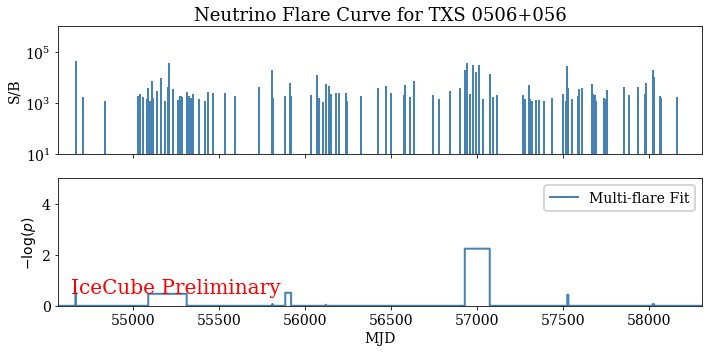
\includegraphics[width=0.8\textwidth]{figs/fcurve_TXS.png}
\caption{The flare curve obtained from the all-sky multi-flare analysis for TXS 0506+056. The pre-trial multi-flare significance of this location is $p=3.37 \times 10^{-4}$ ($3.4 \sigma$). Interestingly, the 2014 flare candidate is not seen at the original significance of $3.5 \sigma$ that was reported in ~\cite{TXS_Multimessenger}. While the 2014 flare candidate is present, this analysis obtains an associated local significance of only $p=0.0054$ ($2.5 \sigma$). }
\label{fig:fcurve_txs}
\end{figure}

\begin{figure}[h]
\centering
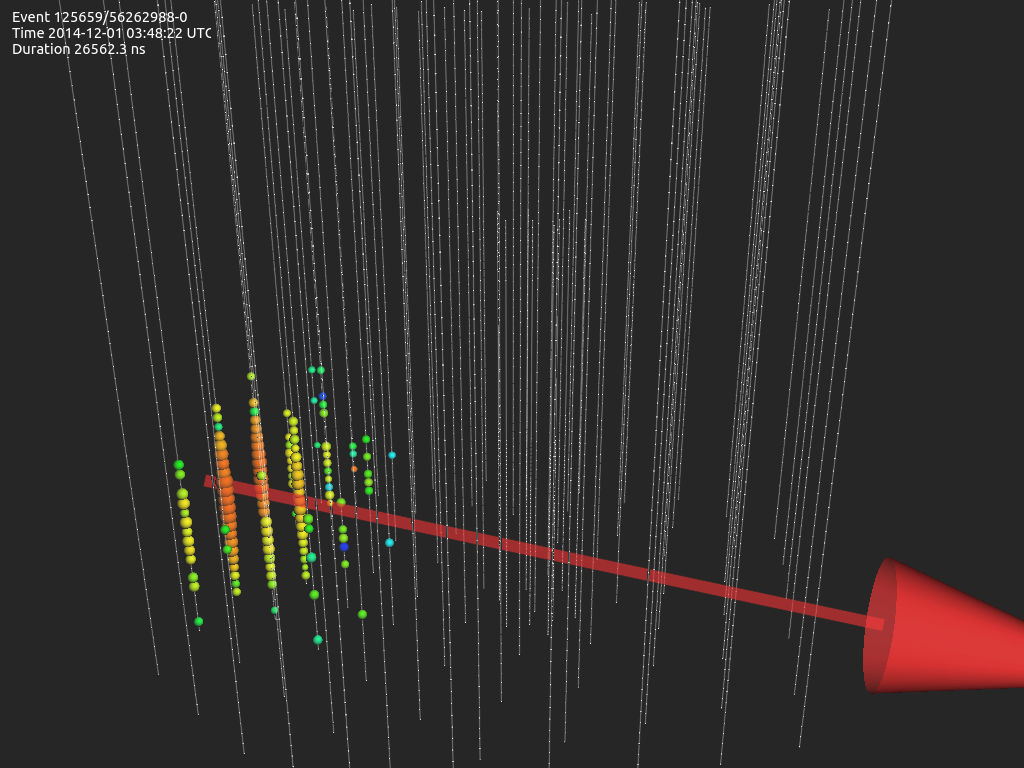
\includegraphics[width=0.45\textwidth]{figs/125659.png}
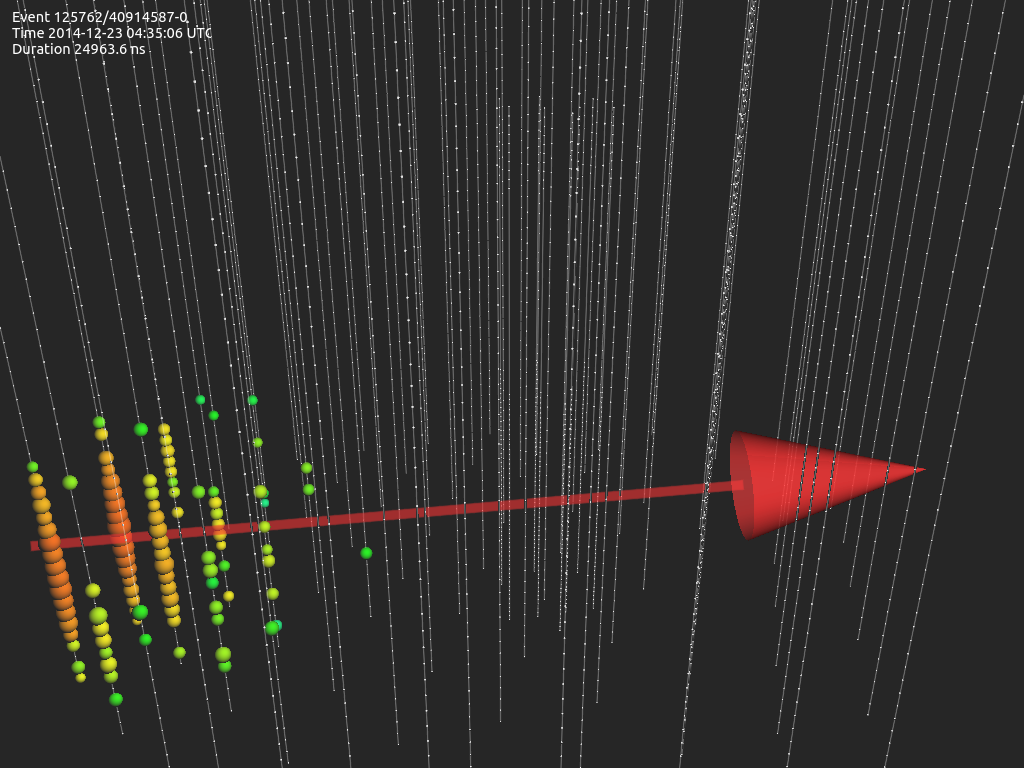
\includegraphics[width=0.45\textwidth]{figs/125762.png}
\caption{The two cascade-like events (event IDs: 40914587 and 56262988) that contributed to the 2014 TXS 0506+056 neutrino flare candidate in PointSourceTracks v002p03, but are not present in PointSourceTracks v003p02. The red arrows show the directional reconstruction assocaited with the track reconstruction that was used, however given the cascade topology of these events, this reconstruction is likely to be inaccurate. }
\label{fig:missingevts}
\end{figure}

As a result of the track length precut that was introduced in PointSourceTracks v003p02, two events (referred to by their event IDs: 40914587 and 56262988) that were major contributors to the 2014 TXS 0506+056 neutrino flare candidate were removed. These events have a cascade-like topology, though in PointSourceTracks v002p03, they are reconstructed as if they were tracks, leading to potentially inaccurate descriptions of the event direction and energy. Since these events are cascade-like, they have a short reconstructed track length, and as such these events do not exist in PointSourceTracks v003p02. 

Manually removing the two cascade events from the PointSourceTracks v002p03 data sample and recomputing the significance of the 2014 TXS 0506+056 neutrino flare results in a drop in significance comparable to what was seen when using PointSourceTracks v003p02, as can be seen in table~\ref{tab:TXSCrossChecks}. The drop in significance cannot be otherwise adequately explained by changes to the angular reconstruction or other differences between the two versions of the data sample. The time-integrated sensitivity of the two samples is comparable, and favors PointSourceTracks v3 at the declination of TXS 0506+056. As such, the drop in significance of the 2014 TXS 0506+056 flare candidate is unlikely to have been caused by PointSourceTracks v003p02 being an overall less sensitive sample.

\begin{table*}[h]
\centering
\begin{tabular}{cccccc}
\multicolumn{6}{c}{Untriggered Flare Cross-check Results} \\[0.1cm]
\hline
\hline
Sample & $p$ (pre-trial) & $T_\text{start}$ & $T_\text{stop}$ & $n_s$ & $\gamma$ \\ 
\hline
\texttt{PSTracks v2}~\cite{TXS_Archival} & 7.0e-5 & 56937.81 & 57096.22 & 14.39 & 2.20  \\
\texttt{PSTracks v2} w/o cascades & 1.17e-3 & 56937.81 & 57112.65 & 12.22 & 2.26 \\
\texttt{PSTracks v3} (multi-flare skymap) & 5.4e-3 & 56927.86 & 57072.99 & 11.87 & 2.22\\
\hline
\hline
\end{tabular}
\caption[]{The results of repeating the untriggered flare analysis preformed in~\cite{TXS_Archival}, but using {\tt PSTracks v3} in place of {\tt PSTracks v2}, the dataset that was originally used. The apparent drop in significance when using {\tt PSTracks v3} can be explained by cascade-like events present in {\tt v2} that have been removed from {\tt v3}.}\label{tab:TXSCrossChecks}
\end{table*}


\begin{figure}[h]
\centering
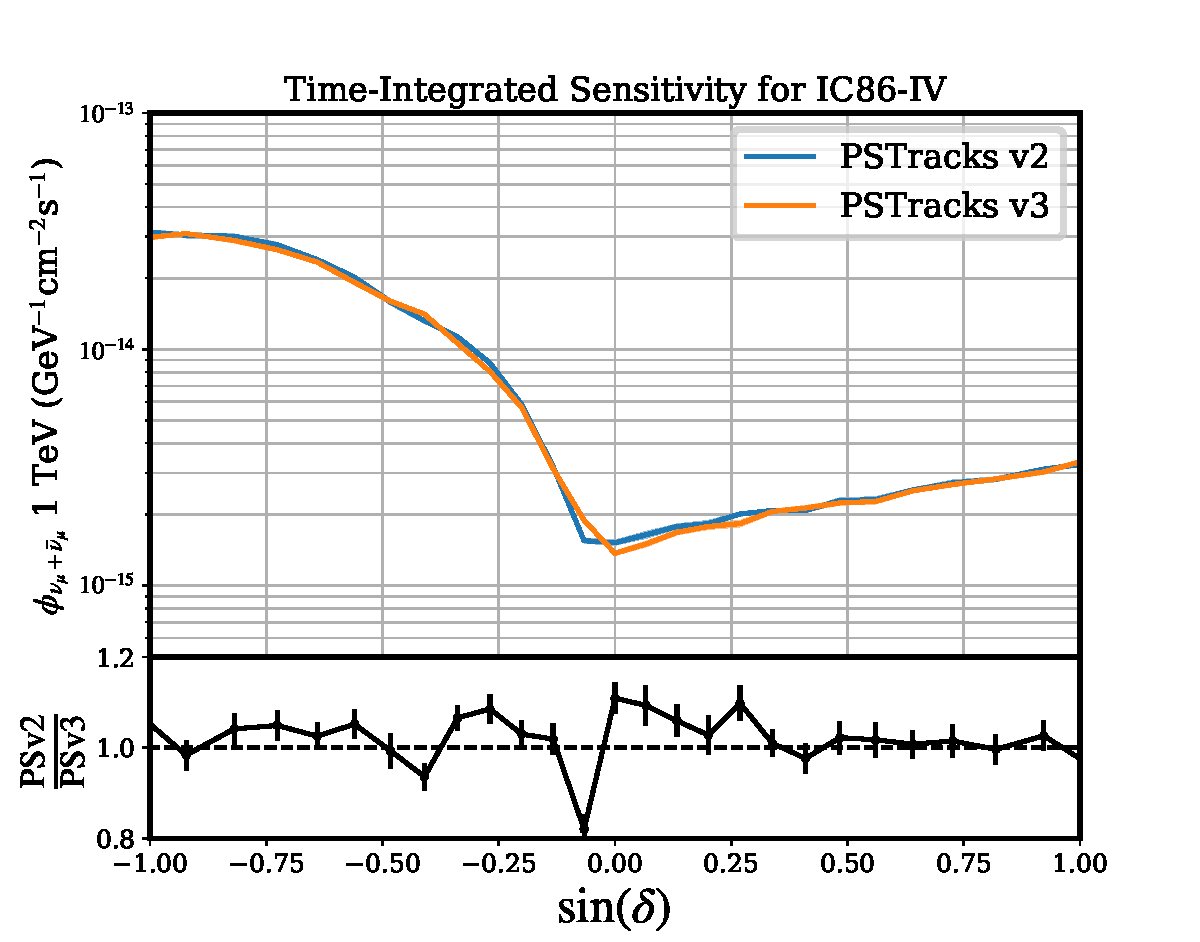
\includegraphics[width=0.8\textwidth]{figs/v2v3_senscompare.pdf}
\caption{A comparison of the time integrated sensitivities of PointSourceTracks v002p03 and PointSourceTracks v003p02. At the declination of TXS 0506+056 ($\delta=5.7^{\circ}$), PointSourceTracks v003p02 has a slightly better sensitivity. }
\label{fig:fcurve_txs}
\end{figure}

It should be noted that the result published in~\cite{TXS_Archival} is not incorrect, despite using an older data sample that contains unforseen background events. Since the methods used for the original untriggered flare analysis use a data-driven background estimation, the cascade background in PointSourceTracks v002p03 is accounted for in the original $3.5 \sigma$ significance that was reported for the 2014 neutrino flare candidate. 

Though the cascade background is handled differently in the PointSourceTracks v002p03 analysis versus the PointSourceTracks v003p02 analysis, the two results are not inconsistent with one another. Figure~\ref{fig:v2v3diff} shows the results of comparing the results of simulated flares comparable to the 2014 TXS flare injected into both PointSourceTracks v002p03 and PointsourceTracks v003p02.   As the background test statistic distributions for both samples are similar, comparing the test statistic values obtained using each sample is a good proxy for comparing the flare local significance.  For this test, trials of simulated signal at the location of TXS 0506+056 were injected into background maps generated using PointSourceTracks v002p03. The injected signal was chosen to replicate the best fit parameters in the original PointSourceTracks v002p03 untriggered flare analysis~\cite{TXS_Archival}: 13 events with a spectral index of $\gamma=2.2$, injected over a time window of length $\Delta t = 158$ days. A test statistic for each of these PointSourceTracks v002p03 signal trials was then calculated. The same simulated signal events were then injected into background trials generated with PointsourceTracks v003p02, but any events that do not pass the PointSourceTracks v003p02 event selection were removed.  A new PointSourceTracks v003p02 test statistic is then calculated for each of these trials with injected signal. 

Figure~\ref{fig:v2v3diff} shows the results of this crosscheck, showing the distribution of test statistics differences between the v2 and v3 test statistics. While on average the test statistic associated with a signal of this type is higher in PointSourceTracks v003p02, the distribution is rather wide, and it is not uncommon for the PointSourceTracks v003p02 result to be lower significance than the PointSourceTracks v002p03 result. A drop in significance comparable or greater than what was seen in the observed v2 and v3 results ($TS_{v3}-TS_{v2}=11.84$) occurs in 8\% of the simulated trials. 


\begin{figure}[h]
\centering
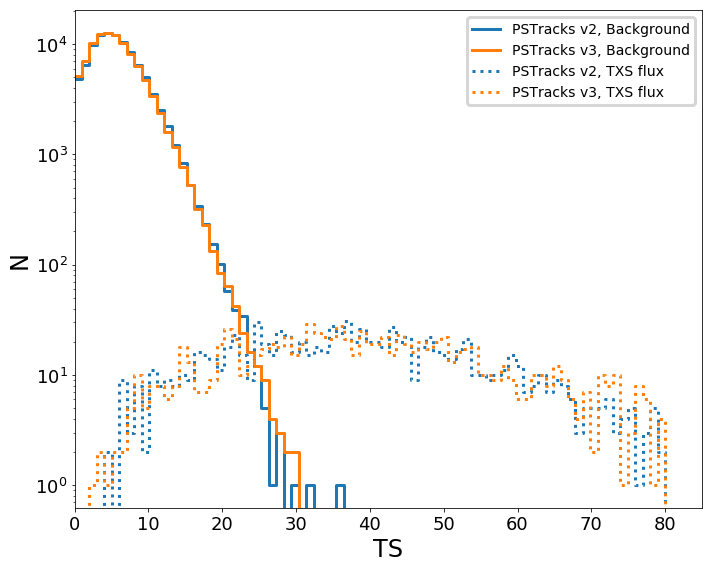
\includegraphics[width=0.4\textwidth]{figs/v2v3tsdists.png}
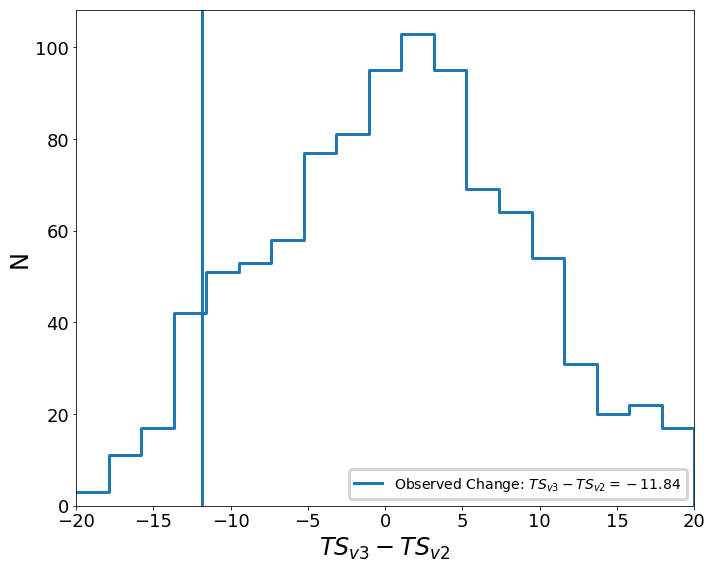
\includegraphics[width=0.4\textwidth]{figs/v2v3tsdiff.png}
\caption{Simulated trials comparing the significance of a flare comparable to the 2014 TXS 0506+056 flare in both PointSourceTracks v002p03 and PointSourceTracks v003p02. Left: the test statistic distributions for both datasets in the background (solid) and injected signal (dotted) cases. The PointSourceTracks v003p02 signal is identical to the PointSourceTracks v002p03 signal, except with events that do not pass the v3 selection removed. Right: A comparison of the v2 and v3 test statistics for each simulated signal trial, with the observed test statistic difference plotted as a vertical line. A drop in significance at least as large as what was seen in observed data occurs in 8\% of simulated trials.}
\label{fig:v2v3diff}
\end{figure}

While there appears to be a drop in significance for the 2014 TXS 0506+056 untriggered neutrino flare when using to the newer PointSourceTracks v003p02 data sample, it is important to realize that the updated v3 result is not inconsistent with the previous v2 result. Additionally, the 2014 flare composes only part of the ensemble of results that make TXS 0506+056 and interesting source candidate, as it is the combination of the 2014 untriggered neutrino flare with the 2017 high energy alert event and multi-messenger observations that suggest TXS 0506+056 as a source of astrophysical neutrinos. The significance of the 2014 TXS 0506+056 flare will likely continue to be monitored as the IceCube collaboration improves its data samples and reconstruction techniques, hopefully converging on a more precise measurement to the flare significance. 


